%<dscrpt>Algèbre linéaire euclidienne : ensemble isogonal.</dscrpt>
On d{\'e}signe par $E$ un espace euclidien dans lequel le produit scalaire de deux vecteurs $x$ et $y$ est not{\'e} $(x/y)$ et la norme d'un vecteur $x$ est not{\'e}e $||x||=\sqrt{(x/ x)}$.\newline
Soit $\alpha\in [-1,1]$, une partie $A$ de $E$ est dite \emph{$\alpha$-isogonale} si et seulement si elle vérifie les conditions suivantes :
\begin{align*}
  &\forall x\in A:\, \Vert x\Vert = 1\\
  &\forall (x,y)\in A^2:\, x\neq y \Rightarrow (x/y)=\alpha
\end{align*}
Une partie est dite \emph{isogonale} si et seulement si elle est $\alpha$-isogonale pour un certain $\alpha$.\newline 
L'objet de ce probl{\`e}me\footnote{premi{\`e}res  parties de l'{\'e}preuve Math2 ENSI de physique 1988} est l'{\'e}tude des parties isogonales.
\subsection*{Partie I. Dans un plan orienté.}
Dans cette partie, $E$ est un espace euclidien orienté de dimension 2. Pour tout r{\'e}el $\theta$, on d{\'e}signe par $r_\theta$ la rotation d'angle $\theta$ dans $E$.
\begin{enumerate}
\item Soit $\alpha\in [-1,1]$, $\theta=\arccos \alpha$ et $x$, $y$ deux vecteurs unitaires de $E$. Montrer que
\begin{displaymath}
(x/y)=\alpha \Leftrightarrow
\left( x=r_\theta (y)\,\text{ ou }\,  y=r_\theta (x)\right) 
\end{displaymath}
\item Soit $\alpha=-\frac{1}{2}$, $\theta=\frac{2\pi}{3}$ et $x$ unitaire. Montrer que $\left\lbrace x,r_\theta (x), r_\theta ^2(x)\right\rbrace$ est $\alpha$-isogonale.
\item L'objet de cette question est de montrer que les parties isogonales définies dans la question précédente sont \emph{les seules} parties isogonales contenant au moins trois éléments.
\begin{enumerate}
\item Soit $\alpha \in [-1,1]$, $\theta =\arccos \alpha$, $A$ une partie $\alpha$-isogonale à trois éléments et $x\in A$.\newline
Montrer que $\theta=\frac{2}{3}\pi$ et que $A=\{x,r_\theta(x),r_\theta^2(x)\}$.
\item  Soit $A$ une partie $\alpha$-isogonale à trois éléments et $B$ une partie $\alpha$-isogonale contenant $A$. Montrer que $B=A$. Conclure.
\end{enumerate}
\end{enumerate}
\subsection*{Partie II. En dimension 3.}
\begin{figure}[ht!]
 \centering
 \includegraphics{./Eisogo_1.pdf}
 % Eisogo_1.pdf: 0x0 pixel, 0dpi, 0.00x0.00 cm, bb=
 \caption{Parties isogonales.}
 \label{fig:Eisogo_1}
\end{figure}

Dans cette partie, $E$ est euclidien de dimension $3$.
\begin{enumerate}
\item Soit $\beta\in [-1,+1]$ et $A=\{u_1,\cdots, u_k\}$ une partie $\beta$-isogonale à $k$ éléments avec $k\geq 4$. On veut montrer que $k=4$ et $\beta=-\frac{1}{3}$.\newline
Pour $i\in\{1,\cdots,k-1\}$, on note $v_i$ le projeté orthogonal de $u_i$ sur le plan orthogonal à $u_k$ (noté $H$) et $w_i=\frac{1}{\Vert v_i\Vert}v_i$.
\begin{enumerate}
\item Montrer que $\beta \in ]-1,1[$.
\item Donner une expression de $v_i$ et calculer les $(v_i/v_j)$.
\item Montrer que $k=4$ et $\beta=-\frac{1}{3}$.
\end{enumerate}
\item Dans cette question, on veut \emph{construire} une partie isogonale à $4$ éléments.\newline
Soit $G$ un sous-espace de dimension 2 de $E$ et $t$ un vecteur unitaire orthogonal {\`a} $G$. Soit $\{u,v,w\}$ une partie $-\frac{1}{2}$-isogonale de $G$. Pour tout couple $(\mu,\nu)$ de r{\'e}els, on pose
\begin{displaymath}
A_{\mu,\nu}=\{t,\mu u+\nu t,\mu v+\nu t,\mu w+\nu t\} 
\end{displaymath}
D{\'e}terminer les couples $(\mu,\nu)$ de r{\'e}els tels que $A_{\mu,\nu}$ soit $-\frac{1}{3}$-isogonale.
\end{enumerate}
\subsection*{Partie III. En dimension quelconque}
Dans cette partie $E$ est euclidien de dimension $n\geq3$.\newline
Pour tout entier $k\geq 2$ et pour tous r{\'e}els $a$ et $b$, on d{\'e}signe par $P_k(a,b)$ la matrice {\`a} $k$ lignes et $k$ colonnes dont tous les termes diagonaux sont {\'e}gaux {\`a} $a$ et tous les termes non diagonaux sont {\'e}gaux {\`a} $b$.\newline
Dans la première question, il peut être utile de considérer les colonnes
\begin{displaymath}
 \begin{pmatrix}
  1 \\ 1 \\ \vdots \\ 1
 \end{pmatrix}
,
 \begin{pmatrix}
  1 \\ 0 \\ \vdots \\ 0
 \end{pmatrix}
,
 \begin{pmatrix}
  0 \\ 1 \\ \vdots \\ 0
 \end{pmatrix}
,\cdots
,
 \begin{pmatrix}
  0 \\ 0 \\ \vdots \\ 1
 \end{pmatrix}
\end{displaymath}
\begin{enumerate}
\item Calculer le d{\'e}terminant de $P_k(a,b)$.
\item Soit $k\geq 3$ et $\{u_1,\cdots,u_k\}$ un ensemble $c$-isogonal. Montrer que 
\begin{displaymath}
\forall (\lambda_1,\cdots,\lambda_k)\in \R^k : \lambda_1 u_1 + \cdots +\lambda_ku_k=0_E 
\Rightarrow
P_k(1,c)
\begin{pmatrix}
 \lambda_1 \\ \vdots \\ \lambda_k         
\end{pmatrix}
=
\begin{pmatrix}
 0 \\ \vdots \\ 0         
\end{pmatrix}
\end{displaymath}
En d{\'e}duire que si $c$ est different de 1 et de $-\frac{1}{k-1}$, les vecteurs $u_1,\cdots,u_k$ constituent une partie libre de $E$.
\item Montrer que toute partie isogonale contient au plus $\dim E +1$ éléments.
\end{enumerate}

\subsection*{Partie IV. Tétraèdre isogonal et transformations}
\begin{figure}[ht!]
 \centering
 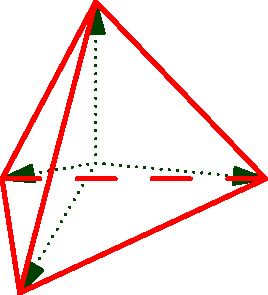
\includegraphics{./Eisogo_2.pdf}
 % Eisogo_2.pdf: 0x0 pixel, 0dpi, 0.00x0.00 cm, bb=
 \caption{Tétraèdre isogonal}
 \label{fig:Eisogo_2}
\end{figure}
Dans cette partie, $B=\{u_1,u_2,u_3,u_4\}$ est un ensemble $-\frac{1}{3}$-isogonal dans un espace $E$ euclidien de dimension $3$.
\begin{enumerate}
\item Montrer que trois vecteurs de $B$ deux {\`a} deux distincts forment une base de $E$. Quelles sont les composantes du vecteur $u_4$ dans la base $\{u_1,u_2,u_3\}$ ?
\item Montrer que pour tout $x$ de $E$, il existe un unique quadruplet $(m_1,m_2,m_3,m_4)\in \R^4$ tel que
\[ \sum_{i=1}^4 m_i=1 \quad \text{et} \quad x=\sum_{i=1}^4m_iu_i\]
On dira que $m_1$, $m_2$, $m_3$, $m_4$ sont les \emph{coordonnées barycentriques} de $x$ dans $B$.
\item On d{\'e}signe par $T$ l'ensemble des vecteurs dont les coordonnées barycentriques dans $B$ sont positives ou nulles. Soit $f$ un automorphisme orthogonal de $E$. On se propose de d{\'e}montrer 
\begin{displaymath}
 f(B)=B \Leftrightarrow f(T)=T
\end{displaymath}
\begin{enumerate}
\item Montrer que $f(B)=B \Rightarrow f(T)=T $.
\item On suppose $f(T)=T$, soit $u\in B$ et $v=f(u)$.\newline
Pourquoi $v$ est-il {\'e}l{\'e}ment de $T$?\newline
On note $(m_1,m_2,m_3,m_4)$ la famille des coordonnées barycentriques de $v$. Montrer que
\[||v||^2=\sum_{i=1}^4m_i^2-\frac{2}{3}\sum_{1\leq i < j \leq  4}m_im_j\]
Calculer
\[\left( \sum_{i=1}^4m_i \right)^2-||v||^2\]
et montrer que
\[\sum_{1\leq i < j \leq 4}m_im_j=0\]
En d{\'e}duire qu'il existe un entier $i$ entre 1 et 4 tel que $m_i=1$ et que les autres $m_j$ soient nuls. Conclure.
\end{enumerate}
\item On d{\'e}signe par $G$ le groupe des bijections de $B$ sur $B$. Soit $\sigma$ un {\'e}l{\'e}ment de $G$.
\begin{enumerate}
\item Montrer qu'il existe un unique endomorphisme $\overline{\sigma}$ du $\R$-espace vectoriel $E$ tel que $\overline{\sigma}(u_i)=\sigma(u_i)$ pour $i=1,2,3$.
\item Montrer que $\overline{\sigma}$ est un automorphisme orthogonal de $E$.
\item Montrer que  $\overline{\sigma}(u_4)=\sigma(u_4)$.
\item Montrer que l'ensemble $\mathcal{G}$ des automorphismes orthogonaux $g$ de $E$ tels que $g(T)=T$ est un sous-groupe du groupe orthogonal de $E$.\newline
Montrer que l'application qui {\`a} $g\in \mathcal{G}$ associe la restriction de $g$ {\`a} $B$ est un isomorphisme de groupe de $\mathcal{G}$ vers $G$. Quel est le cardinal de $\mathcal{G}$?
\item Pour tout couple $(i,j)$ d'entiers distincts entre 1 et 4, on d{\'e}signe par $H_{i,j}$ le plan vectoriel orthogonal {\`a} $u_i-u_j$ et par $\tau_{i,j}$ la r{\'e}flexion par rapport {\`a} $H_{i,j}$. Utiliser l'isomorphisme entre $\mathcal{G}$ et $G$ pour montrer que tout
{\'e}l{\'e}ment de $\mathcal{G}$ est une composition d'un nombre fini de $\tau_{i,j}$.
\end{enumerate}
\end{enumerate}
